\chapter{Conclusion}

In this chapter, we summarize our contributions in the thesis and present some
future extensions.
% - Recall contributions with more details assuming someone has read it
%
% - Future work (chapter by chapter)
\section{Contributions}

In this thesis, we have developed some tools to better understand and make use
of the computations happening within complex systems.
We summarize our contributions below.

\begin{itemize}
  \item In Chapter \ref{cha:background}, we gave an overview of the \acf{CA}
        model and the specific challenges it poses. We review the deep
        connection between \acp{CA} and \acfp{RNN} and how this leads to using
        \acp{CA} in \acf{RC}. Next, in chapter \ref{cha:literature-review}, we
        place our work within the large body of literature on complex systems,
        complexity, emergence and learning.

  \item In Chapter \ref{cha:meas-compl-evolv}, we define a novel metric of
        complexity for complex systems. The metric is inspired by principles of
        compression, and algorithmic complexity. It uses the ability of small
        neural networks to learn a model of the local structures in a system,
        and the evolution of the predictive power of that model as the system
        evolves over time. We evaluate the quality of this metric by measuring
        its correlation with the perception of complexity of humans. We find a
        higher correlation with human annotations than alternative methods on a
        dataset of \acp{CA} rules labeled as complex or not. We use the metric
        to discover new \acp{CA} rules with surprisingly complex behavior
        semi-automatically.

  \item In Chapter \ref{cha:visu-comp-large}, we built on the work of Chapter
        \ref{cha:meas-compl-evolv} to work on the specific challenges posed by
        working with large-scale systems such as cellular automata. In these
        systems, qualitatively different behavior may emerge at various scales.
        To allow dealing with these large systems and apply complexity measures
        and classification methods on a range of scales, we developed three
        coarse-graining methods based on simple statistical analysis, clustering
        algorithms and autoencoder neural networks, that can reduce the size of
        a system while retaining useful information.

  \item In Chapter \ref{cha:learn-effic-compl}, we tackled the issue of using
        complex systems for general purpose task solving, using the \ac{RC}
        paradigm. We also developed a metric for the speed of learning of
        machine learning systems. Using that metric, we looked at the data
        efficiency of some well know algorithms rather than their task-based
        performance only. Surprisingly, \ac{RC} models using random frozen
        \acp{RNN} or \acp{CA} are significantly more efficient that other
        alternatives on a range of tasks. We evaluated this on some standard
        language datasets and introduced our own dataset of progressively more
        complex tasks. Efficiency is a crucial property in low data and compute
        settings, and our work showed that some overlooked methods may actually
        be competitive in these situations.
\end{itemize}

\section{Future Work}

This thesis has explored the connections between learning, complex systems, and
open-ended evolution. These fields are not young but many open problems still
remain, some of them poorly understood, making this research exploratory in
nature. We hope our work can advance our understanding of learning and
adaptation in natural and artificial systems, leading to the development of more
effective and efficient learning algorithms in the future.

\subsection{Evolving cellular automata for complexity}

The metric of complexity developed in Chapter \ref{cha:meas-compl-evolv} and the
others presented in Section \ref{sec:measuring-complexity} often give a single
value output from a system's evolution over time. Similar to how
\textcite{mitchellEvolvingCellularAutomata1996} evolves \acp{CA} rules to solve
a particular task, it seems appealing to use the complexity as a fitness
function for a genetic algorithm. Such an algorithm would generate new rules
that are progressively more complex (according to the complexity metric).

It is hard to apply this principle in practice. Because complexity metrics are
often approximating some uncomputable ideal metric, results get less satisfying
as we maximizing a particular metric. This could be accounted for in future
works using multiple complementary complexity metrics, or using other surrogate
metrics, such as the ability to learn to solve auxiliary tasks and generalize.
This approach motivated our work from Chapter \ref{cha:learn-effic-compl}, where
we design a benchmark of progressively more complex tasks that could be used to
evaluate the ability of a system to perform complex computations.

\subsection{Feedback reservoir computing}

In Chapter \ref{cha:learn-effic-compl}, we explored the applications of the
\ac{RC} paradigm to \acp{CA}. In general, \ac{RC} assumes a purely forward
model, meaning that inputs are fed to the reservoir and outputs are decoded from
it. The trainable decoder layer is trained offline on a training dataset and
tested next. We illustrate the \ac{RC} principle in figure
\ref{fig:classical_reservoir}. This structure is often sufficient for supervised
tasks when a sufficiently large training dataset is available.

\begin{figure}[htbp]
  \centering
  \begin{subfigure}[t]{.5\linewidth}
    \centering
    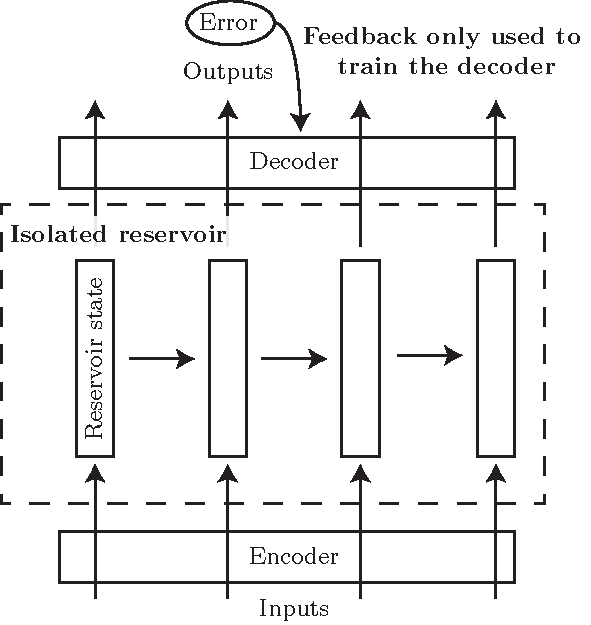
\includegraphics[width=\linewidth]{figures/classical_reservoir.pdf}
    \caption{Classical reservoir computing}
    \label{fig:classical_reservoir}
  \end{subfigure}
  \begin{subfigure}[t]{.45\linewidth}
    \centering
    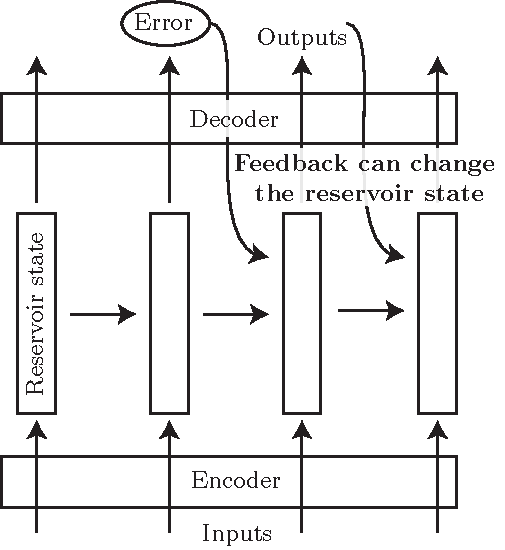
\includegraphics[width=\linewidth]{figures/feedback_reservoir.pdf}
    \caption{Feedback reservoir computing}
    \label{fig:feedback_reservoir}
  \end{subfigure}
  \caption{Comparison of regular reservoir computing with feedback reservoir
    computing.}
  \label{"waiting for reftex-label call..."}
\end{figure}

A straightforward extension that could make \ac{RC} systems fully autonomous
would be to feed back and error signal within the reservoir state at each
output. This extension we call \emph{feedback reservoir computing} is
illustrated in figure \ref{fig:feedback_reservoir} alongside the standard
\ac{RC} model \ref{fig:classical_reservoir}. An ideal system would adapt to this
error signal to adjust future outputs through some internal learning algorithm,
progressively improving itself. The only mechanism that should be built into
this system would be an incentive to minimize received error signals through
adaptation. The main limitation to this idea is the design of such a system with
built-in adaptation is not easy. We do not know of a mechanism that can enable
autonomous adaptation and improvement without any external input. Our work on
complex systems points towards cellular automata and other complex systems as
candidates for supporting such a mechanism, which would rely on growth of
complexity.

\subsection{Learning in dynamical systems}

By examining the process of learning in complex systems, neural networks, and
the reservoir computing framework from a unified perspective, we are able to
identify a generalization that provides a valuable perspective on the problem of
learning in dynamical systems. This generalization allows us to consider the
various components of these systems in a more integrated manner, enabling us to
develop a more comprehensive understanding of the underlying mechanisms of
learning without having to focus on a particular dynamical system.

This form of learning occurs dynamically as a system is simulated or run. Rather
than utilizing traditional parameter updates, it takes place in the system's
state or ``activations'', resulting in what we refer to as \emph{learning in
  dynamical systems}. This process is analogous to an inner loop or ``thinking''
phase, during which the system can self-organize by manipulating its current
state without external changes to its parameters. This type of learning is
already present in various machine learning systems, including some \acfp{RNN},
which use short-term dynamical learning to solve language-based tasks (see
Section \ref{sec:dynam-learn-acprnn}). It is also present in some form in the
\ac{RC} framework, and the update rule of gradient-based learning algorithms.
While effective, this form of learning is often not studied or optimized to the
same extent as more conventional methods of parameter optimization.

\paragraph{Generic model}\label{sec:generic-model}
We give a general description of a model of learning in dynamical systems. A
dynamical systems is described by a sequence of variables $S_{t}$ taking values
in some state space $\mathcal{S}$ at times indexed by $t$. In the most general setting the
state space can be real-valued or discrete and the time index may also be
continuous or discrete. An evolution function $f$ specifies the state of the
dynamical system at time $t$ given a history of states for $t' < t$. It may be
deterministic or stochastic.

We study the special case of discrete-time dynamical systems, where the current
state depends on the previous state.

\begin{equation}
  \forall t \in \mathbb{N},\quad S_{t + 1} = f(S_{t})
  \label{eq:dyn-update}
\end{equation}

Inputs can be used to condition the update rule and enable the dynamical system
to interact with an environment.

\begin{equation}
S_{t+1} = f(S_t, x).
\label{eq:11}
\end{equation}

An output can be observed from the current state $S_t$ with a decoding function
$D$. We define the output for time step $t$,
\begin{equation}
  \label{eq:10}
  y_t = D(S_t).
\end{equation}
Depending on the use cases, alternate representations may be considered where
the output depends on two or more timesteps or an input vector $x$.
We give a few well-known examples of learning in dynamical systems from the
field of machine learning.

\paragraph{Dynamical learning in \acp{RNN}}\label{sec:dynam-learn-acprnn}
We study the example of a question answering task with a pre-trained \ac{RNN}.
It is easy to see that a \ac{RNN} can be fully written using \eqref{eq:11} and
\eqref{eq:10}. The task of question answering is about reading information from
a prompt and answering a question that involves recalling some data from the
prompt. An example of such prompt and question:
\begin{equation*}
  \underbrace{\texttt{Two cats and five dogs sleep on the red mat.}}_{\text{Prompt}}
  \underbrace{\texttt{How many dogs are there?}}_{\text{Question}}
\end{equation*}
More advanced question answering requires reasoning and advanced processing of
the prompt. In the example above, it would be enough to remember words from the
prompt.

We consider a trained \ac{RNN} evaluated on a question answering test set. If
the dataset was designed in a correct way, the network should have no prior
information about a sentence/question pair before reading it. The prompt's
relevant piece of information has to be stored within the values of the hidden
state of the \ac{RNN} and not in the neural network weights since they are not
being changed during this phase. This transient learning which enables the
\ac{RNN} to memorize the beginning of the prompt is exactly the type of
dynamical learning we describe above. The \ac{RNN} was trained to achieve this,
but once it is trained, learning happens dynamically.

Modern \acp{RNN} are not designed to take full advantage of this memory
property, and will progressively overwrite memory if ran for more timesteps.
Still, they illustrate the type of learning we want to emphasize. We expect
advanced systems to not only be able to keep that memory, but also be capable of
manipulating stored information to reason about and form novel concepts.

\paragraph{Supervised learning with stochastic gradient descent}
\label{sec:superv-learn-with}
We consider another example: a single hidden layer neural network with weight
matrices $W_1 \in \mathbb{R}^{n \times d}$ and $W_2 \in \mathbb{R}^{d \times o}$. We train the network with
standard backpropagation and stochastic gradient descent with learning rate $\tau$.
The neural network is represented with a function $F$ and the loss function
between the network outputs and label is written $\mathcal{L}$.

Using the notations from Section \ref{sec:generic-model}, we define
$S_{t} = \left(W_{1}^{(t)}, W_{2}^{(t)}\right) \in \mathbb{R}^{n \times d} \times \mathbb{R}^{d \times o}$
containing the neural network parameters at step $t$ of the training. We assume
the training pairs $(X_{k}, y_{k})$ are numbered according to their selection
order for the stochastic gradient descent algorithm.

The stochastic gradient update function for the state $S_{t}$ is:
\begin{equation}
  \label{eq:supervised-learning}
  S_{t+1} = {f}(S_t, X_t, y_t) = \left(W_1^{(t)} - \tau \frac{\partial
      \mathcal{L}(F(X_t), y_t)}{\partial W_1^{(t)}}, W_2^{(t)} - \tau \frac{\partial
      \mathcal{L}(F(X_t), y_t)}{\partial W_2^{(t)}} \right).
\end{equation}

Note that the function $f$ is deterministic for a given ordering of the training
pairs. The stochasticity of $f$ is thus contained in the numbering of the
training examples.

\begin{figure}[ht]
  \centering
  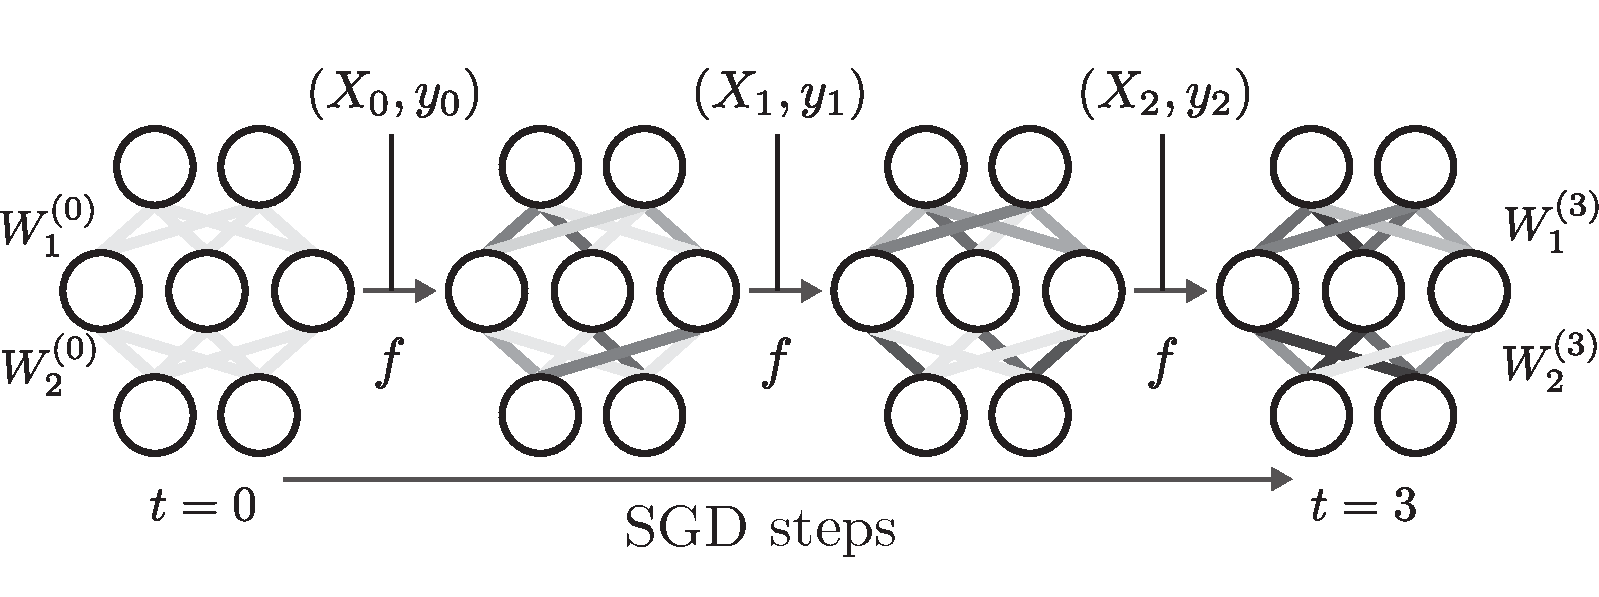
\includegraphics[width=.9\linewidth]{figures/learning_nn.pdf}
  \caption{\label{fig:label} Learning happens within the ``activations'' of this
    dynamical system, which in this example are the weights of the neural
    network. The fixed update function depends on an input pair $(X, y)$
    and the previous state vector $S = (W_1, W_2)$.}
\end{figure}

We note that $f$ is a fixed update function (using a dynamical system point of
view of the training pipeline, a training input/output pair $(X, y)$ is a pair
of input values). In supervised learning, the function $f$ makes the state
converge to a fixed point. This property is desired when solving a target task
characterized by the loss $\mathcal{L}$. Because of that convergence property a neural
network cannot be expected to produce any novel behavior after the end of its
training. On the contrary, we know that other complex dynamical systems that we
study in this thesis like cellular automata may exhibit behavior of increasing
complexity during their development, with no sign of convergence towards a
stable state.
